\documentclass[../Cours.tex]{subfiles}

\begin{document}
\clearpage

\color{black}

\begin{center}
    \Huge{Épreuves communes de $4^{\mbox{ème}}$}
\end{center}

\begin{questions}

\EXERCICE{12}
Chaque question ne contient \textbf{qu'une seule bonne réponse}, et ne nécessite \textbf{aucune justification}.

\begin{center}
\begin{tabularx}{\linewidth}{|l|C|C|C|C|} \hline 
    Question & A & B & C & D \\\hline \hline 
    \makecell{Quelle est la mesure de l'angle, \\sachant que les deux droites sont parallèles ?\\
    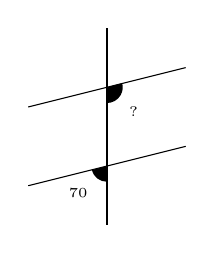
\begin{tikzpicture}
        \draw (0,0) -- (2,0.5);
        \draw (0,-1) -- (2,-0.5);
        \draw (1,1) -- (1,-1.5);
        \fill[black] (1,-0.75) -- ++(0,-0.2) arc(-90:-165:0.2) node[midway,below left]{\tiny{\ang{70}}} -- cycle;
        \fill[black] (1,0.25) -- ++(0,-0.2) arc(-90:15:0.2) node[midway,below right]{\tiny{?}} -- cycle;
    \end{tikzpicture}} & \ang{70} & \ang{110} & \ang{20} & \ang{50}\\ \hline
    \makecell[l]{La décomposition en \\facteurs premiers de $210$ est :} & $21 \times 10$ & $2 \times 3 \times 5 \times 7$ & $5 \times 6 \times 7$ & $3 \times 70$ \\\hline
    \makecell[l]{Une boisson est composée de sirop et d’eau dans \\la proportion d’un volume de sirop pour sept \\volumes d’eau (c’est-à-dire dans le ratio 1:7).\\ La quantité d’eau nécessaire pour préparer \\\qty{560}{\milli\litre} de cette boisson est...} & \qty{70}{\milli\litre} & \qty{80}{\milli\litre} & \qty{400}{\milli\litre} & \qty{490}{\milli\litre} \\\hline
    \makecell[l]{Soit la série de nombres \{15 ; 10 ; 13 ; 9 ; 10 ; $x$\}\\ La moyenne de la série est 11 pour $x$ égal à ...} & 8 & 9 & 10 & 11 \\\hline
\end{tabularx}
\end{center}

\EXERCICE{16}
Albert fait du vélo au col de la Croix de Fer.\\
Il est parti d'une altitude de \qty{589}{\metre} et arrivera au sommet à une altitude de \qty{2064}{\metre}.
Sur le schéma ci-dessous, qui n'est pas en vraie grandeur, le point de départ sera représenté par le point $D$ et le sommet par le point $S$.

\begin{center}
    \begin{tikzpicture}
        \draw (0,0) node[below left]{$D$} -- (4,0) node[right]{$H$} node[midway,below] {distance horizontale} -- (4,3) node[above right]{S} node[midway,right]{dénivelé} -- cycle;
        \node[rotate=37] at (1.7,1.9) {route de \qty{28.28}{\kilo\metre}};
        \draw[dashed] (0,0) -- (-6,0);
        \node[anchor=east] at (-3,1) {\scriptsize{Saint Jean de Maurienne}};
        \node[anchor=east] at (-3,0.5) {\scriptsize{(altitude : \qty{589}{\metre})}};
        \draw[dashed] (4,3) -- (10,3);
        \node[anchor=west] at (7,4) {\scriptsize{Col de la Croix de Fer}};
        \node[anchor=west] at (7,3.5) {\scriptsize{(altitude \qty{2064}{\metre})}};
        \draw[fill=black] (4,0) rectangle +(-0.25,0.25);
    \end{tikzpicture}
\end{center}

\question Déterminer le dénivelé $SH$.
\question Calculer la distance horizontale $DH$.

\clearpage
\EXERCICE{20}
Voici deux programmes de calcul.

\begin{center}
    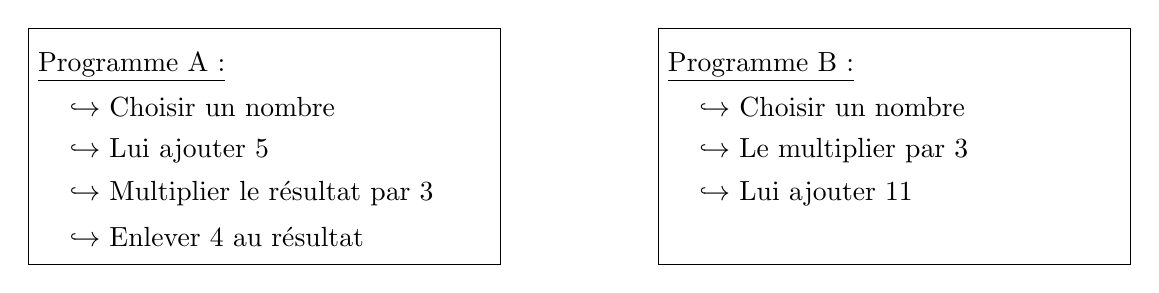
\begin{tikzpicture}
        \draw (0,0) rectangle +(6,3);
        \draw (8,0) rectangle +(6,3);
        \node[anchor=west] at (0,2.5) {\underline{Programme A :}};
        \node[anchor=west] at (8,2.5) {\underline{Programme B :}};
        \node[anchor=west] at (0.4,2) {$\hookrightarrow$ Choisir un nombre};
        \node[anchor=west] at (0.4,1.45) {$\hookrightarrow$ Lui ajouter 5};
        \node[anchor=west] at (0.4,0.9) {$\hookrightarrow$ Multiplier le résultat par 3};
        \node[anchor=west] at (0.4,0.35) {$\hookrightarrow$ Enlever 4 au résultat};
        \node[anchor=west] at (8.4,2) {$\hookrightarrow$ Choisir un nombre};
        \node[anchor=west] at (8.4,1.45) {$\hookrightarrow$ Le multiplier par 3};
        \node[anchor=west] at (8.4,0.9) {$\hookrightarrow$ Lui ajouter 11};
    \end{tikzpicture}
\end{center}

\question 
    \subquestion Réaliser les deux programmes de calcul en choisissant 10.
    \subquestion Réaliser les deux programmes de calcul en choisissant -2.
\question Que remarque-t-on ?
\question 
    \subquestion Réaliser les deux programmes de calcul en choisissant $x$.
    \subquestion Montrer que les deux expressions littérales obtenues sont égales.

\EXERCICE{20}
Le futuroscope est un parc de loisirs situé dans la Vienne. L'année 2019, il a enregistré \num{1.9} millions de visiteurs.

\question Combien aurait-il fallu de visiteurs en plus en 2020 pour atteindre 2 millions de visiteurs ?
\question L'affirmation << Il y a eu environ \num{5200} visiteurs par jour en 2019 >> est-elle vraie ?
\question Deux élèves de 3e, Marie et Adrien, se souviennent avoir vu en mathématiques que les hauteurs inaccessibles pouvaient être déterminées avec l’ombre d'un objet ou d'une personne. \\
Ils souhaitent calculer la hauteur de la Gyrotour du Futuroscope.\\
Marie se place comme indiquée sur la figure ci-dessous, de telle sorte que son ombre coïncide avec celle de la tour. Après avoir effectué plusieurs mesures, Adrien effectue le schéma ci-dessous (le schéma n’est pas à l’échelle), sur lequel les points $A$, $E$ et $B$ ainsi que les points $A$, $D$ et $C$ sont alignés. \\
\textbf{Calculer la hauteur $BC$ de la Gyrotour.}

\begin{center}
    \begin{tikzpicture}
        \coordinate (A) at (0,0);
        \coordinate (B) at (8,4);
        \coordinate (C) at (8,0);
        \coordinate (E) at ($(A)!0.4!(B)$);
        \coordinate (D) at ($(A)!(E)!(C)$);
        \draw (A) -- (B) -- (C) -- cycle;
        \draw (D) -- (E) node[midway,above,rotate=90]{Marie};
        \node[left] at (A) {$A$};
        \node[above] at (B) {$B$};
        \node[below] at (C) {$C$};
        \node[above] at (E) {$E$};
        \node[below] at (D) {$D$};
        \node[above,rotate=90] at ($(B)!0.5!(C)$) {gyrotour};
        \draw[Latex-Latex] (C) ++(0.2,0) -- ++(0,4) node[midway,right]{?};
        \draw[Latex-Latex] ($(A)+(0,-0.2)$) -- ($(D)+(-0.2,-0.2)$) node[midway,below]{\qty{2}{\metre}};
        \draw[Latex-Latex] ($(D)+(0.2,-0.2)$) -- ($(C)+(-0.2,-0.2)$) node[midway,below]{\qty{54.25}{\metre}};
        \draw[Latex-Latex] ($(D)+(0.2,0.1)$) -- ($(E)+(0.2,0)$) node[midway,below,rotate=90]{\qty{1.60}{\metre}};
        \draw[dashed] (E) -- +(1,0);
    \end{tikzpicture}
\end{center}

\clearpage
\EXERCICE{20}

\textbf{Document 1}
\begin{centre}
    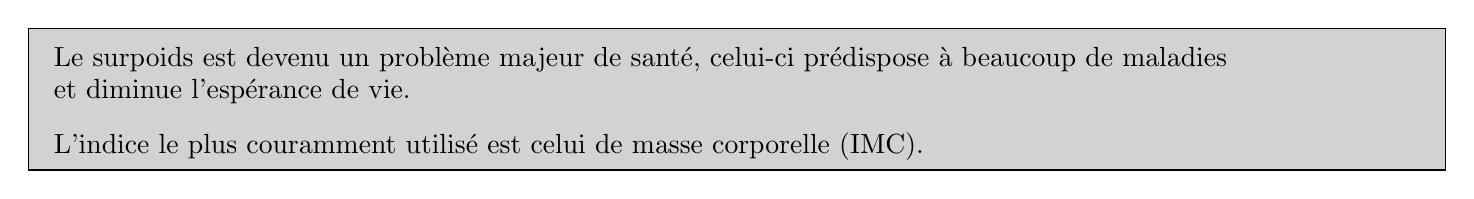
\begin{tikzpicture}
        \draw[fill=lightgray!70!white] (0,0) rectangle (18,1.8);
        \node[anchor=west] at (0.2,1.4) {Le surpoids est devenu un problème majeur de santé, celui-ci prédispose à beaucoup de maladies};
        \node[anchor=west] at (0.2,1) { et diminue l’espérance de vie.};
        \node[anchor=west] at (0.2,0.3) {L’indice le plus couramment utilisé est celui de masse corporelle (IMC).};
    \end{tikzpicture}
\end{centre}

\textbf{Document 2}
\begin{centre}
    \begin{tikzpicture}
        \draw[fill=lightgray!70!white] (0,-0.1) rectangle (18,3.5);
        \node[anchor=west] at (0.2,3.1) {L’IMC est une grandeur internationale permettant de déterminer la corpulence d’une personne };
        \node[anchor=west] at (0.2,2.7) {adulte entre 18 ans et 65 ans.};
        \node[anchor=west] at (0.2,1.7) {Il se calcule avec la formule suivante : $\mbox{IMC} = \dfrac{\mbox{masse}}{\mbox{taille}^2}$ ~~~~ avec << masse >> en \unit{\kilo\gram} et << taille >> en \unit{\metre}.};
        \node[anchor=west] at (0.2,1) {\textbf{Normes :~~~~} $\num{18.5} \infeg \mbox{IMC} < 25$ ~~~~corpulence normale};
        \node[anchor=west] at (2.45,0.6) {$25 \infeg \mbox{IMC} < 30$ ~~~~surpoids};
        \node[anchor=west] at (2.45,0.2) {$\mbox{IMC} \supeg 30$ ~~~~obésité};
    \end{tikzpicture}
\end{centre}

\question Dans une entreprise, lors d’une visite médicale, un médecin calcule l’IMC de six des employés. Il utilise pour cela une feuille de tableur dont voici un extrait :

\begin{center}
    \begin{tabularx}{0.9\linewidth}{c|c|C|C|C|C|C|C|}\hline
       \rowcolor{lightgray!50!white} & A & B & C & D & E & F & G \\ \hline 
       1 & Taille (en \unit{\metre}) & \num{1.69} & \num{1.72} & \num{1.75} & \num{1.78} & \num{1.86} & \num{1.88} \\\hline
       2 & Masse (en \unit{\kilo\gram}) & 72 & 85 & 74 & 70 & 115 & 85\\\hline
       3 & IMC (*) & \num{25.2} & \num{28.7} & \num{24.2} & \num{22.1} & \num{33.2} & \num{24.0} \\\hline
       4 & \multicolumn{2}{|c|}{\scriptsize{\textit{(*) valeur approchée au dixième}}} &&&&&\\\hline
    \end{tabularx}
\end{center}

\subquestion Combien d’employés sont en situation de surpoids ou d’obésité dans cette entreprise ?
\subquestion Laquelle de ces formules a-t-on écrite dans la cellule B3, puis recopiée à droite, pour calculer l’IMC ? \textbf{Recopier la formule correcte sur la copie.}

\begin{center}
    \hfill\boxed{= 72/1.69\^{}2} \hfill \boxed{= B1 / (B2 * B2) } \hfill \boxed{= B2 / (B1 * B1) } \hfill \boxed{= \$B2 / (\$B1*\$B1)}\hfill
\end{center}

\question Le médecin a fait le bilan de l’IMC de chacun des 41 employés de cette entreprise. Il a reporté les informations recueillies dans le tableau suivant dans lequel les IMC ont été arrondis à l’unité près.

\begin{center}
    \begin{tabularx}{0.8\linewidth}{|c|*{8}{C|}c|}\hline
        IMC & 20 & 22 & 23 & 24 & 25 & 29 & 30 & 33 & Total \\\hline
        Effectif & 9 & 12 & 6 & 8 & 2 & 1 & 1 & 2 & 41 \\\hline
    \end{tabularx}
\end{center}

\subquestion Calculer l’IMC moyen, arrondi à l'entier près, des employés de cette entreprise.
\subquestion Quel est l’IMC médian ? 
\subquestion On lit sur certains magazines : << On estime qu’au moins \qty{5}{\%} de la population mondiale est en surpoids ou est obèse >>. Est-ce le cas pour les employés de cette entreprise ?

\EXERCICE{12}
Léo a ramassé des fraises pour faire de la confiture.
\question Il utilise les proportions de sa grand-mère : \qty{700}{\gram} de sucre pour \qty{1}{\kilo\gram} de fraises.\\
Il a ramassé \qty{1.8}{\kilo\gram} de fraises. \textbf{De quelle quantité de sucre a-t-il besoin ?}
\question Après cuisson, Léo a obtenu \qty{2.7}{\litre} de confiture.
Il verse la confiture dans des pots cylindriques de \qty{6}{\centi\metre} de diamètre et de \qty{12}{\centi\metre} de haut, qu’il remplit jusqu’à \qty{1}{\centi\metre} du bord supérieur.\\
\textbf{Combien pourra-t-il remplir de pots ?}\\[1ex]
Rappels : $\qty{1}{\litre}=\qty{1000}{\centi\metre\cubed}$ ~~ Volume d’un cylindre = $\pi \times r^2 \times h$

\end{questions}
\end{document}